\documentclass[letterpaper, 11pt]{article}
\usepackage{latexsym}
\usepackage{amssymb}
\usepackage{times}
%\usepackage[in]{fullpage}
\usepackage{amsmath,amsfonts,amsthm}
\usepackage{graphicx}
\usepackage{fullpage}
\usepackage{graphicx}
\usepackage{caption}
\usepackage{subcaption}
\usepackage{cite}
%\usepackage{algorithm2e}
\usepackage{algorithm}
%\usepackage{algorithmic}
\usepackage{algpseudocode}
%%%%%%%DEMO ALGORITHMICX %%%%%%%%%%%%%%%%%%%%%%
%\begin{algorithm}
%\caption{Euclid�s algorithm}\label{euclid}
%\begin{algorithmic}[1]
%\Procedure{Euclid}{$a,b$}\Comment{The g.c.d. of a and b}
%\State $r\gets a\bmod b$
%\While{$r\not=0$}\Comment{We have the answer if r is 0}
%\State $a\gets b$
%\State $b\gets r$
%\State $r\gets a\bmod b$
%\EndWhile\label{euclidendwhile}
%\State \textbf{return} $b$\Comment{The gcd is b}
%\EndProcedure
%\end{algorithmic}
%\end{algorithm}

%\documentclass[11pt]{article}
%\pagestyle{myheadings}
%\usepackage[ruled,nothing]{algorithm}
%\usepackage{algorithmic}
%\usepackage[dvips]{epsfig,graphicx}
%\numberwithin{equation}{section}

\bibliographystyle{plain}

\newenvironment{newalgo}[2]{\begin{algorithm}

\caption{\textsc{#1}}\label{#2}

\begin{algorithmic}[1]}{\end{algorithmic}\end{algorithm}}



\newcommand{\gm}{\gamma}
\newcommand{\wh}{\widehat}
\newcommand{\rep}{representation}
\newcommand{\rv}{random variable}
\newcommand{\la}{\lambda}
\newcommand{\wt}{\widetilde}
\newcommand{\st}{such that}
\newcommand{\slvary}{slowly varying}
\newcommand{\ma}{moving average}
\newcommand{\regvary}{regularly varying}
\newcommand{\asy}{asymptotic}
\newcommand{\ts}{time series}
\newcommand{\id}{infinitely divisible}
\newcommand{\seq}{sequence}
\newcommand{\fidi}{finite dimensional \ds}

\newcommand{\ble}{\begin{lemma}}
\newcommand{\ele}{\end{lemma}}
\newcommand{\bfX}{{\bf X}}
\newcommand{\pro}{probabilit}
\newcommand{\BX}{{\bf X}}
\newcommand{\BY}{{\bf Y}}
\newcommand{\BZ}{{\bf Z}}
\newcommand{\BV}{{\bf V}}
\newcommand{\BW}{{\bf W}}
\newcommand{\reals}{{\mathbb R}}
\newcommand{\bbr}{\reals}

\newcommand{\balpha}{\mbox{\boldmath$\alpha$}}
\newcommand{\bbeta}{\mbox{\boldmath$\beta$}}
\newcommand{\bmu}{\mbox{\boldmath$\mu$}}
\newcommand{\tbmu}{\mbox{\boldmath${\tilde \mu}$}}
\newcommand{\bEta}{\mbox{\boldmath$\eta$}}


\def \br#1{\left \{#1 \right \}}
\def \pr#1{\left (#1 \right)}

\newcommand{\Gm}{\Gamma}
\newcommand{\ep}{\epsilon}


\newtheorem{lemma}{Lemma}[section]
\newtheorem{figur}[lemma]{Figure}
\newtheorem{theorem}[lemma]{Theorem}
\newtheorem{proposition}[lemma]{Proposition}
\newtheorem{definition}[lemma]{Definition}
\newtheorem{corollary}[lemma]{Corollary}
\newtheorem{example}[lemma]{Example}
\newtheorem{exercise}[lemma]{Exercise}
\newtheorem{remark}[lemma]{Remark}
\newtheorem{fig}[lemma]{Figure}
\newtheorem{tab}[lemma]{Table}
\newtheorem{fact}[lemma]{Fact}
\newtheorem{test}{Lemma}

\newcommand{\play}{\displaystyle}

\newcommand{\ms}{measure}
\newcommand{\beao}{\begin{eqnarray*}}
\newcommand{\eeao}{\end{eqnarray*}\noindent}
\newcommand{\beam}{\begin{eqnarray}}
\newcommand{\eeam}{\end{eqnarray}\noindent}

\newcommand{\halmos}{\hfill\mbox{\qed}\\}
\newcommand{\fct}{function}
\newcommand{\ins}{insurance}
\newcommand{\ds}{distribution}

\newcommand{\one}{{\bf 1}}
\newcommand{\eid}{\buildrel{\rm d}\over {=}}
\newcommand {\Or}{\rm ORDER}
\newcommand {\In}{\rm INTER}

\newcommand{\bbd}{{\mathbb D}}
\newcommand{\vi}{$V_{ij}$ }
\newcommand{\rr}{R^{\prime\prime}}
%\newcommand{\R}{R^\prime}
\newcommand{\ci}{\frac{1}{c}}
\newcommand{\Vi}{V(n)}
\newcommand{\dR}{\mathcal R}
\newcommand{\md}[1]{\left(\ \rm{mod}\ \it{#1}\right)}
\newcommand{\So}{s}
%\begin{document}
%\def\DoubleSpace{\baselineskip=24pt}
%\DoubleSpace \sloppy

\begin{document}



\title{Machine Translation en600.468 \\ Decoding }
\author{Adithya Renduchintala and Aric Velbel}
\maketitle

\section{Introduction}
For the decoding challenge, we deciding to use finite state machinary to build a
decoding pipeline. Our system consists of 4
Finite state automata:\\
\begin{itemize}
  \item A source language Phrase segmentation FST
  \item A phrase translation FST
  \item Target language Phrase to Token FST
  \item A target languare language model
\end{itemize}
The phrase translation model and the language model are weighted FSTs. The
weights for these FSTs were the log probabilities that accompanied the
translation table and the language model.\\
To obtain a translation, the following steps were followed.\\
\begin{itemize}
  \item Convert an input source language string to a FSA $S$.
  \item Compose $S$ with the Phrase Segmentation FST, $P$, to obtain a FST that
  represents all possible segmentations of the input sentence.
  \item The result of the previous composition was composed with the translation
  FST $Tr$.
  \item The result of that was composed with the target language Phrase to
  Tokens FST $Pt$.
  \item The result of that composition was finally composed with the language
  model FST $L$.
  \item Each path in the final machine $F$ represents a possible translation,
  the path with the least weight was chosen as the winning translation. The output
  symbols along the best path is the output translation string.
\end{itemize} 
The composition expression the above sequece is:\\
\begin{align*}
F &= S \circ P \circ Tr \circ Pt \circ L\\
T_w &= min(F)\\
\end{align*}
Here $T_w$ is the output symbols along the best path in machine $F$. The
topology of each of these FSTs will be described in further detail in the
sections below.
\section{Phrase Segmentation}
To create a source phrase segmentions, we used the translation table. For each
phrase on the source side in the table, we add an arc $a$, in our FST. The input
symbols along $a$ are the individual tokens of the phrase. The output symbol is
the concatenation of each of the tokens in the phrase. For e.g. the phrase
\emph{absolument pas} would be concatenated as \emph{absolument\_pas}, but
alternate segmentations could also exist, in this example it is possible that
the two words are not concated into a single phrase, but get modeled as 2
phrases each with one token. This example is illustrated in \ref{fig:segment1}
and \ref{fig:segment2}.\\
\begin{center}
	\begin{figure}
	\begin{subfigure}[a]{\textwidth}
    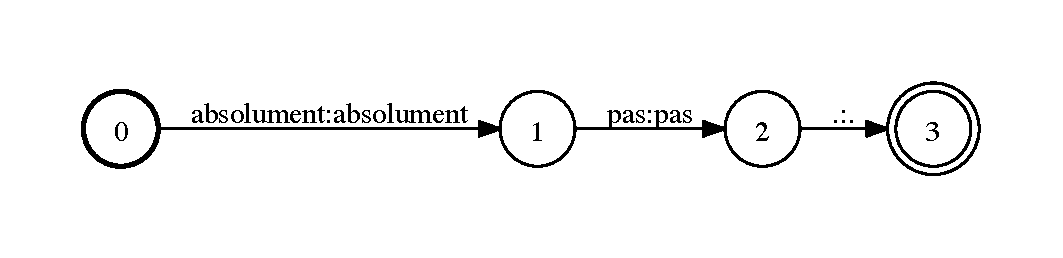
\includegraphics[width=\textwidth]{lc.pdf}
    \caption{input sentence FSA}
     \label{fig:segment1}
    \end{subfigure}
    \begin{subfigure}[b]{\textwidth}
    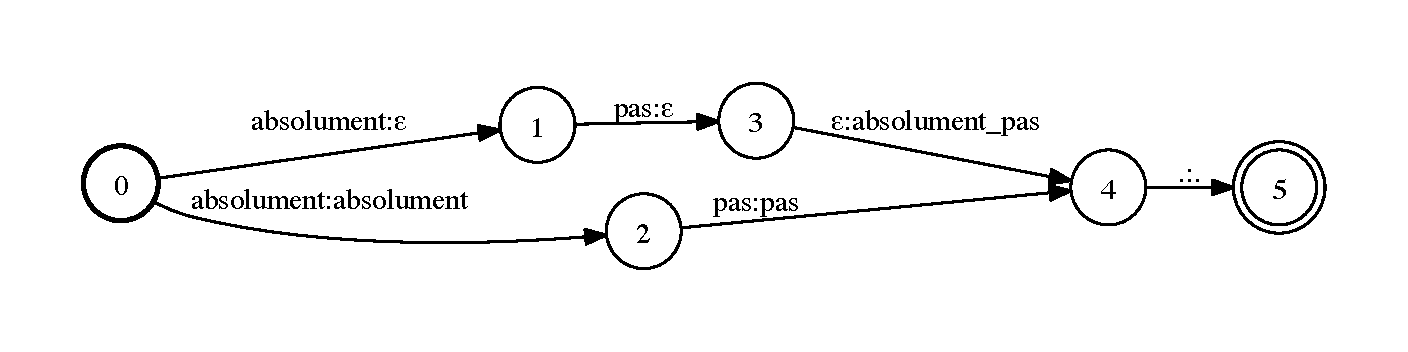
\includegraphics[width=\textwidth]{lc-seg.pdf}
    \caption{input sentence composef with segmenation FST}
    \label{fig:segment2}
    \end{subfigure}
    \end{figure}
\end{center}
\section{Translation}
The translation fst is a single state FST, with multiple arcs. Each arc has
input and output symbols from each entry in the translation table. The weight of
the arc is the negative of the log probability associated.\\
\section{Tokenization}
The symbols that appear in the machine after translation are entire phrases, but
we need the symbols to be in token space so that a language model can be
applied. The tokenization FST simply is the inverse of the phrase segmentation
FST, except for the target language.\\
\section{Language Model}
This machine takes the FST that has been generated so far by all the previous
FSTs. The job of the LM FST is to score each path by how probable the path is in
the target language. We followed the topology used by \cite{Allauzen:2003:GAC:1075096.1075102}. In
this topology each state of the FST represents the context of a token. For a trigram
LM the context is at most 2 previous tokens. The state $w_{i-2}w_{i-1}$
represents the context for the current token $w_i$. Suppose the trigram
$w_iw_{i-1}w_{i-2}$ has not been observed, then we back off from the bigram
context to a unigram context represented by the state $w_{i-1}$. The arc
connecting the bigram context to the unigram context applies the back off
cost$\phi$. Furthermore we can use the same template when backing off from a
unigram context to a 'null' context. This is shown in \ref{fig:lmbk}.
\begin{figure}
\begin{center}
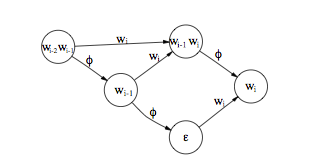
\includegraphics[width=0.5\textwidth]{lm.png}
\caption{Language model with back off transitions, \cite{Allauzen:2003:GAC:1075096.1075102}}
\label{fig:lmbk}
\end{center}
\end{figure}
\subsection{Dealing with unk}
\subsubsection{Removing unk form final translation}
A detail that has not be mentioned so far is how we deal with \emph{unk} tokens.
Since we can look up the translation table for each sentence, we add an arc to
represent a source phrase to \emph{unk} is the source phrase does not exist in the
translation table. This means that the best path could contain \emph{unk} in
the output, but we would like unk to be replaced by the source phrase that we
could not find a translation for. In order to achive this, we simply copy the
input symbol onto the output symbol (when the output symbol is \emph{unk}). This
solution also has a potential problem. The input and output symbols are not
always 'arc aligned'. So merely copying the input symbol might produce incorrect
results. For a input sentence, we maintain a list of tokens $U_{tokens}$ that
are translated as \emph{unk}. When an
\emph{unk} is seen in the output, the closest input symbol that is in $U_{tokens}$
is used as the replacement for \emph{unk}. We recognize that this might not work in
all cases, especially when there are multiple unknown words in a sentences, and
when there is a lot of reordering between source and target, but in this data
set we do not observe those issues.\\
\subsubsection{Back off from unk}
In the ARPA formated language model given, there is no back off weight for the
unk token, and there is not othre bigram (or trigram) that starts with unk.
This presents a issue when modeling the LM FST. Consider reaching reaching the
unk state in the LM FST, with out a back-off or bigrams starting with unk
there are no out going arcs from the state. Thus, no paths from the start to a
final state exist that include the unk state. This made sentences with unknown
words end up with no possible translations. To fix this issue, we added back-off
arc with no cost from the \emph{unk} state to the 'null' state.
\section{Phrase Reordering}
Initial results with the original pipeline did not address the issue of phrases
in the source moving to a different location in the target. To address this, me
agumented our FST cascade with a Phrase Reodering FST $Rp$. This FST does not
permit arbitrary re-ordering as the language resulting from arbitraty re-ordering is
not regular\cite{knight1998translation}. We allow adjacent phrase swaps using a
reordering FST.\\
\begin{align*}
F &= S \circ P \circ Rp \circ Tr \circ Pt \circ L\\
T_w &= min(F)\\
\end{align*} 
The result of composing a input FSA with this FST is
shown in \ref{fig:reorder}.
\begin{center}
\begin{figure}
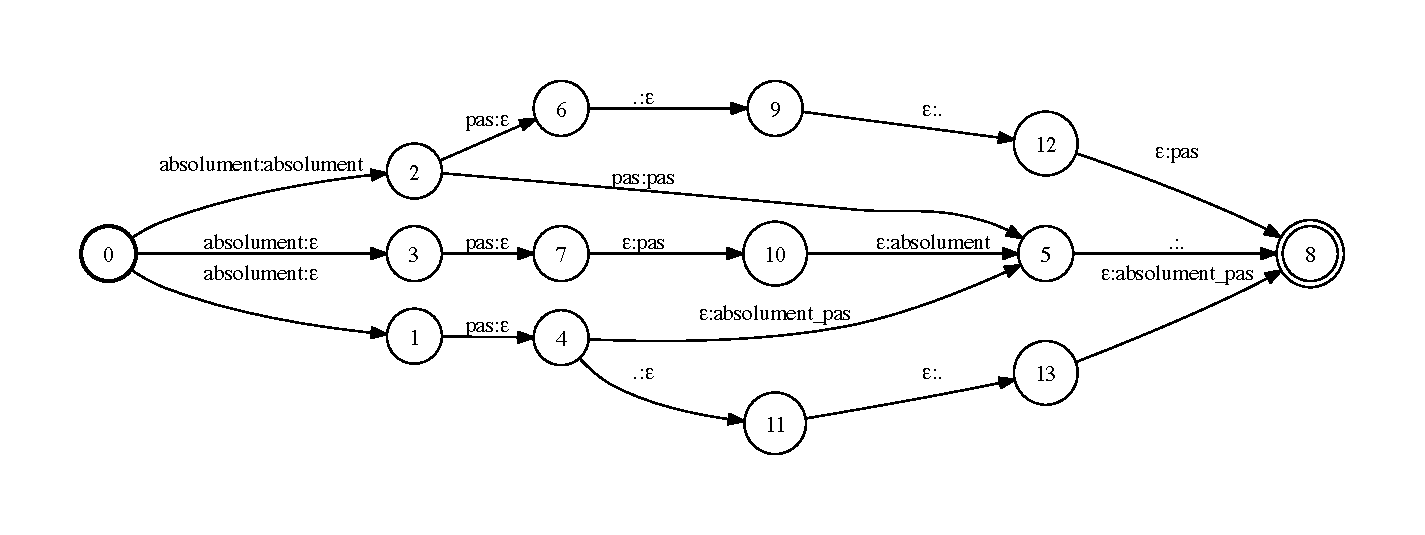
\includegraphics[width=\textwidth]{lc-seg-re.pdf}
\caption{FST obtained after composing segmentation output with phrase
reordering FST}
\label{fig:reorder}
\end{figure}
\end{center}
\section{Result}
The reordering model did better than the no-reordering model, with scores of
-1325 and 1374, but both models failed to score well in the model score metric.
The reason for this is because the FST composition treats the negative log probabilities as weights, so its
possible that translations that score well on the TM model, are rejected because
they do not score well on the LM.Consider the translation of the phrase
\emph{absolument pas}. Let us assign two possible translations to this phrase
\emph{absolutely not} and \emph{no}, with negative log probabilities 0.335 and
1.113. Under the language more \emph{absolutely not} and \emph{no} get scores of
106.741 and 104.856 (including probability of start sentence and end sentence
symbols).So the Language Model gets to reject better translations. This is a
useful feature is most cases, but it appears to not perform well under the model
score metric.There are number of possible ways to improve on this, which we hope
to continue working towards:\\
\begin{itemize}
  \item Learning a score scaling parameter that 'dampens' the effect of the
  language model
  \item Add negative weights to longer phrases to counter the effect of the LM
  favoring shorted sentences
  \item Pruning away paths after the translation model, so that the LM can only
  rescore paths that we know scored well on the translation.
\end{itemize}
Each of these methods involve fine tuning parameter that make the translations
score optimum under both the LM and TM. We tried to manually change such
parameter to get a sence of what values might help, but none of the values we
tried did better than the original cascade. Automating the process and plotting
the result might help get a sence of what range of values these parameters can
take.
\bibliography{bib}{}
\bibliographystyle{plain}
\end{document}



































